\chapter{Diseño Dirigido por el Dominio}

Para el diseño del software he elegido aplicar DDD\textit{(Domain Driven Design)} para enfocar el 
desarrollo del producto en el dominio del problema, de forma que, el sistema contemple el lenguaje y reglas 
del dominio. Este tipo de diseño se centra en el usuario al igual que la metodología ágil, la cual,
también se usa en el proyecto. El potencial de este diseño reside en que se alinea estrechamente el producto
con los conceptos y términos clave del dominio. Sin embargo, tiene algunos inconvenientes para un TFG como
necesitar una comunicación continua e iterativa con expertos del dominio.

\section{Lenguaje Ubicuo}
He creado un glosario con un conjunto de términos pertenecientes al dominio que se emplearán dentro del desarrollo del producto, 
de esta manera cuando se den las reuniones entre los desarrolladores y los expertos de dominios no dará lugar a confusiones, 
ya que, habremos definido con anterioridad las palabras claves.

Estas son algunas definiciones que ayudarán a establecer un lenguaje común entre los expertos de dominio y los
desarrolladores al discutir y codificar las reglas de negocio.
 
\begin{itemize}
\item \textbf{Cita:} Una cita se refiere a una programación de tiempo para que un paciente se encuentre con un médico o profesional de atención primaria en un centro de salud.
\item \textbf{Paciente:} Una persona que busca atención médica en el sistema de atención primaria.
\item \textbf{Médico:} Un proveedor de atención médica que ofrece servicios de atención primaria, como médicos generales o especialistas en medicina familiar.
\item \textbf{Riesgo:} Un valor asociado al cálculo de diferentes factores que implica un mayor peligro cuando alguien enferma
\item \textbf{Centro de salud:} Un sitio físico donde se brinda atención primaria a los pacientes, como un consultorio médico, una clínica o un centro de atención ambulatoria.
\item \textbf{Historia clínica:} Un registro médico que contiene información detallada sobre la salud de un paciente, incluyendo diagnósticos, tratamientos anteriores, alergias y otros datos relevantes.
\item \textbf{Síntomas:} Los signos o manifestaciones físicas que indican una posible enfermedad o condición médica.
\item \textbf{Diagnóstico:} La identificación de una enfermedad o condición médica basada en los síntomas del paciente, exámenes médicos y evaluaciones clínicas.
\item \textbf{Tratamiento:} Las acciones médicas o terapias recomendadas para abordar una enfermedad o condición médica específica.
\item \textbf{Receta:} Una prescripción médica para medicamentos o terapias específicas para ser administradas al paciente.
\item \textbf{Expediente médico:} Un conjunto de registros y documentos relacionados con la atención médica de un paciente, incluyendo historias clínicas, resultados de exámenes, informes de consultas y otros datos importantes.
\end{itemize}

\section{Mapa Contextual}
Mediante la comunicación entre el equipo de desarrollo y los expertos del dominio se dividirá la complejidad del problema
en distintas áreas de las cuales se deben de distinguir: dominio, subdominio y un contexto acotado. Disgregando el dominio 
conseguimos una visión más amplia y simple para cada contexto acotado, de esta forma, podemos enfocarnos en el modelado de
cada dominio diminuyendo la complejidad del dominio principal. A continuación presentaré el mapa contextual ya disgreado con 
las relaciones entre entornos:

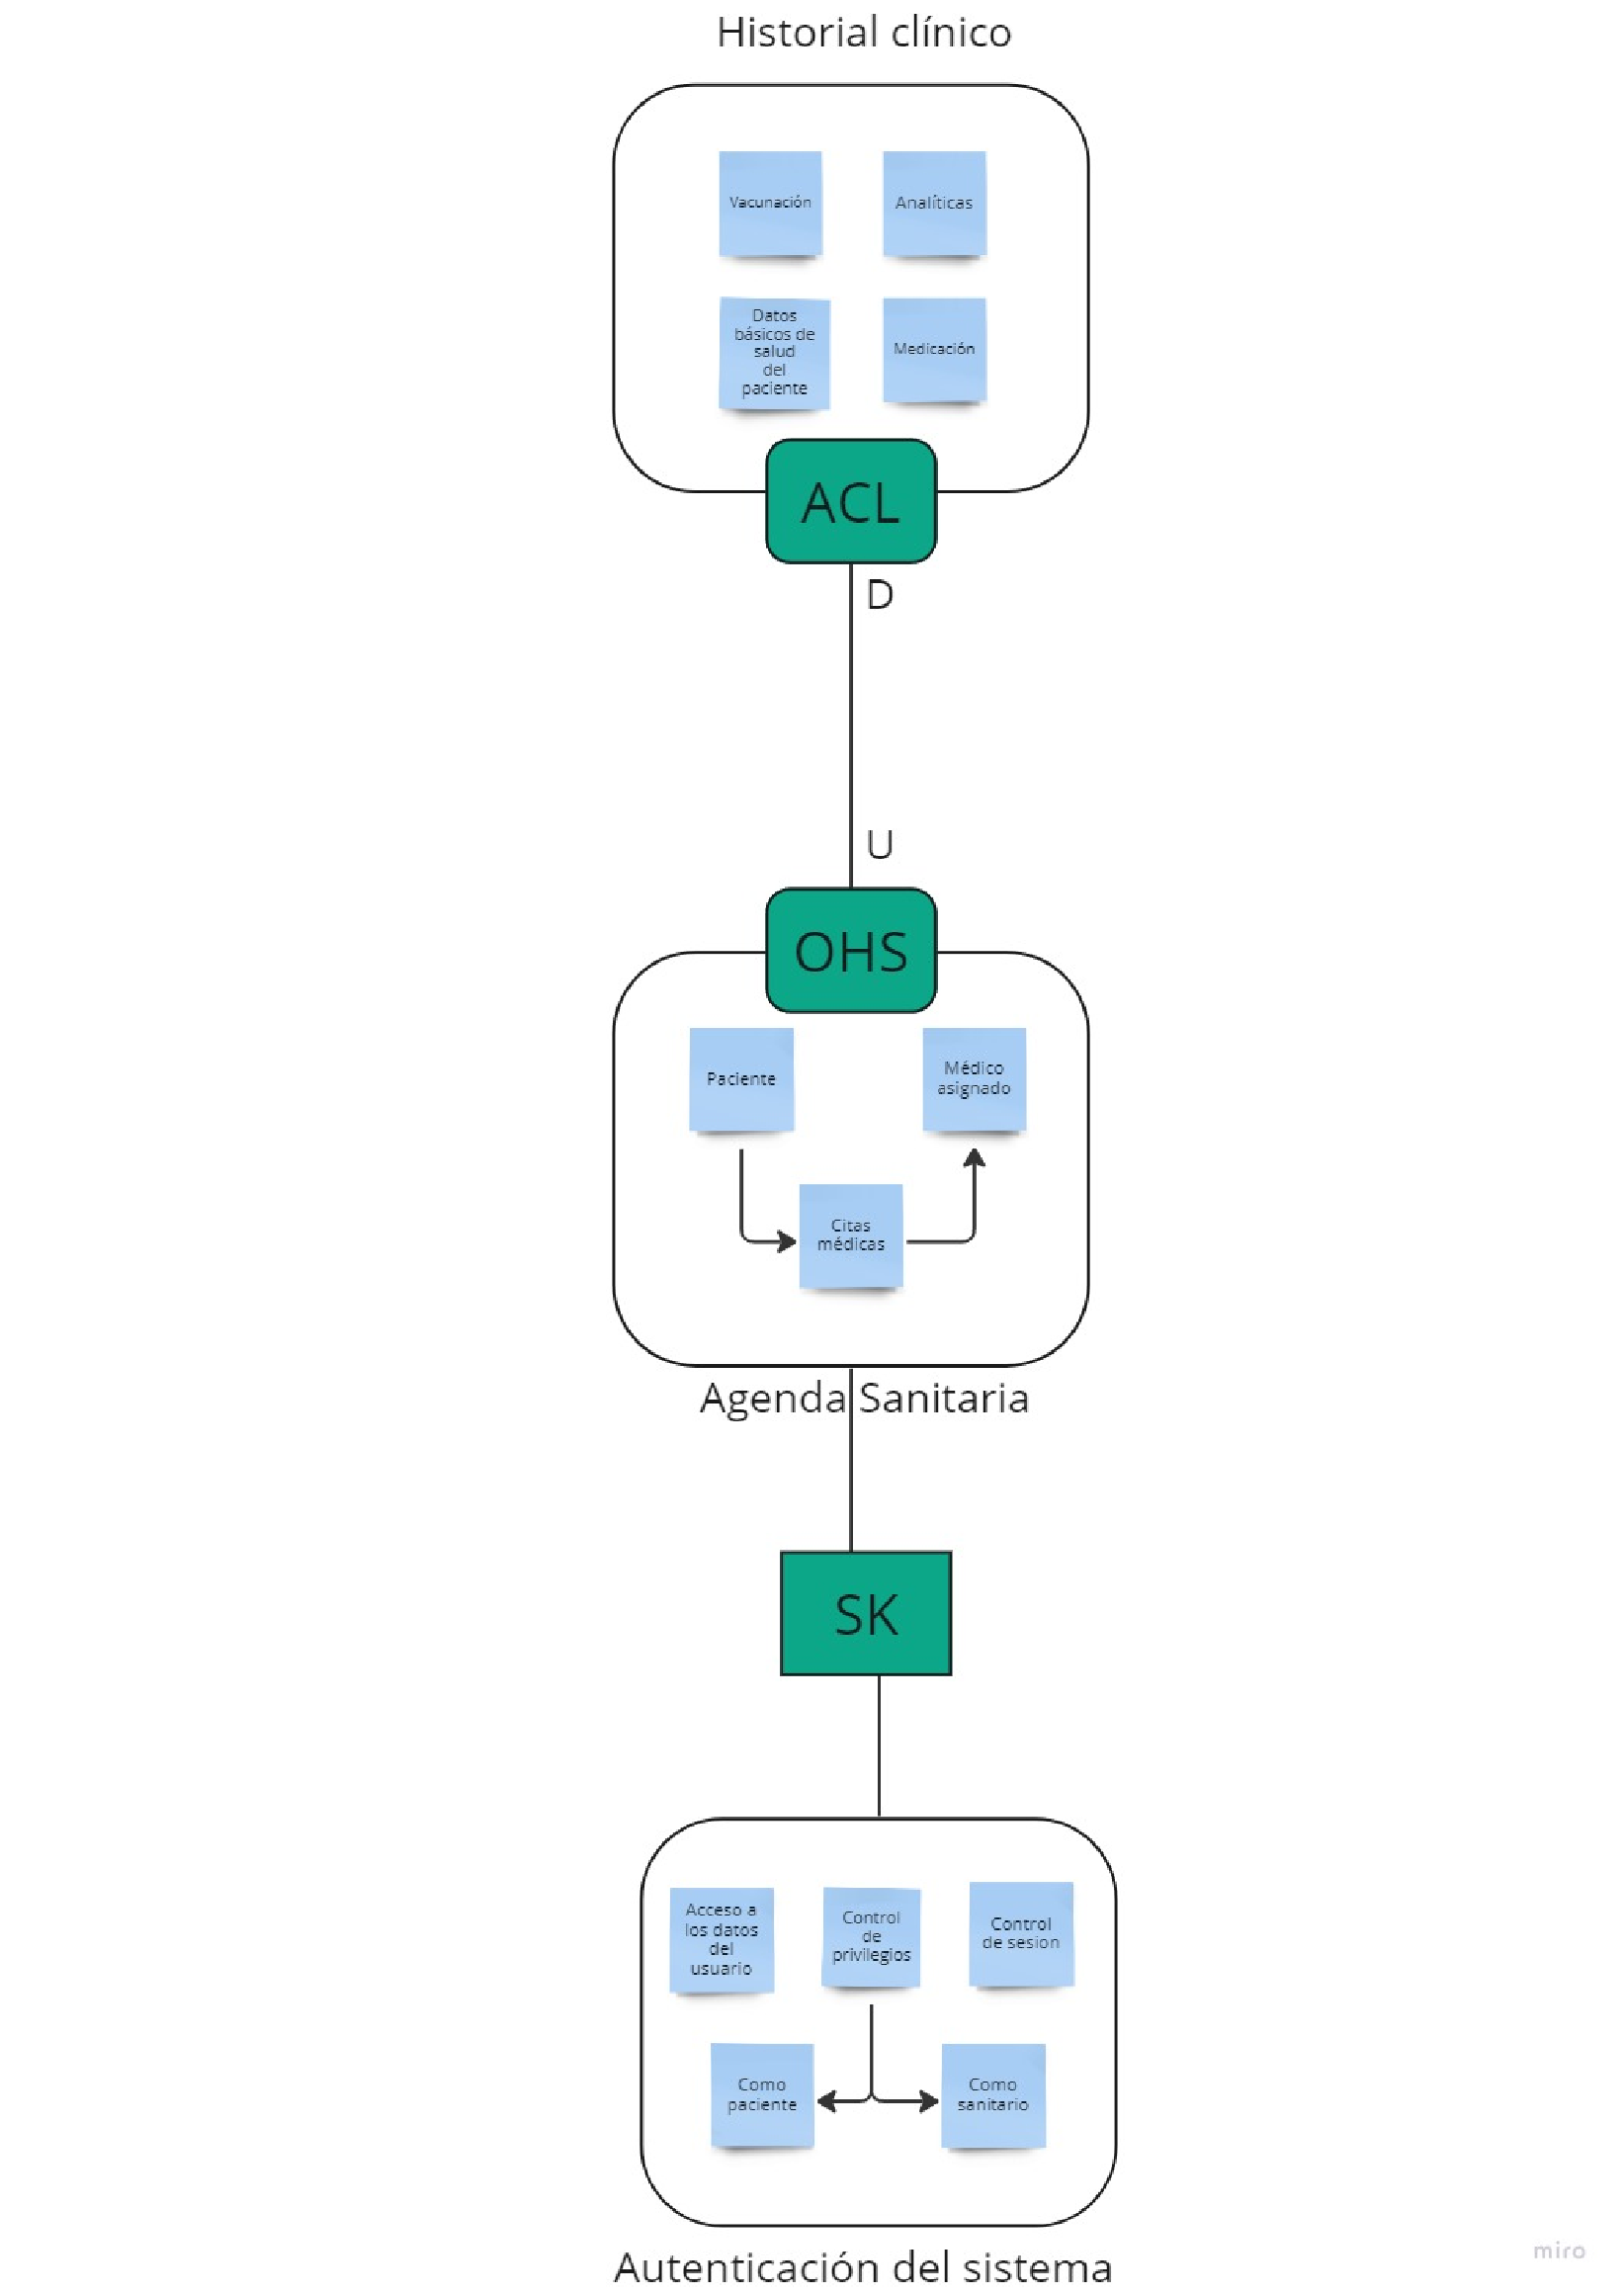
\includegraphics{contextual_map.pdf}

Como podemos observar en la imágen he diferencidado entre tres diferentes contextos que se relacionan entre ellos. 
El principal contexto es la Agenda Sanitaria, la cuál actúa de \textit{(Open Host Service)} para el Historial Clínico del paciente, 
esto implica que el historial vendrá alimentado por el Agenda Sanitaria. Por otra parte el Historial Clínico actúa como 
\textit{(Anticorruption Layer)}, esto significa que se crea una capa extra en el modelado del problema para evitar la corrupción
de datos. Finalmente el Sistema de Autenticación y la Agenda Sanitaria tienen una relación de \textit{(Shared Kernel)}, esto significa
que a pesar de estar en diferentes subdominios comparten parte del código y se retroalimentan. 



Dentro del Diseño Dirigido por el Dominio debemos abstraer distintos módulos para disgregar el problema en pequeñas partes
y componerlo desde los trozos más pequeños posibles de código hasta formar el diseño que resuelva este problema. 
Por esto es necesario dividir en diferentes secciones cada uno de estos módulos y explicarlos por separado.

\section*{Objetos de Valor}
Son un objeto inmutable, usado para representar un valor. Pueden compararse con otros objetos de valor para comprobar 
si tienen los mismos valores representados y no tienen identidad propia. 
Suelen ser la combinación de atributos primitivos que adquieren un significado al leerse juntos, por ello deben encapsularse
en un único objeto de valor, por ejemplo las coordenadas geográficas (latitud y longitud). A veces tiene sentido convertir
un atributo primitivo a objeto de valor, dependiendo del dominio del problema.
Los Objetos de Valor identificados son los siguientes: DNI, N.º de seguridad social, Riesgo, Coordenadas, Código Postal.
Utilizaré el DNI como ejemplo principal: 


\begin{lstlisting}
# app/models/dni.rb
class DNI
    attr_reader :number
  
    def initialize(number)
      validate_number!(number)
      @number = number
    end
  
    def ==(other)
      self.class == other.class && number == other.number
    end
  
    def to_s
      number
    end
  
    private
  
    def validate_number!(number)
      raise ArgumentError, 'Número de DNI inválido' unless 
      valid_format?(number)
    end
  
    def valid_format?(number)
      /^[0-9]{8}[A-Z]$/ === number
    end
  end
\end{lstlisting}

  

